\documentclass[12pt]{article}
\usepackage{tabularx}
\usepackage{float}
\usepackage{booktabs}
\usepackage{colortbl}
\usepackage[table,xcdraw]{xcolor} % enables \rowcolor and more
\usepackage{subcaption}
\usepackage{graphicx}
\usepackage{caption}
\usepackage{mathrsfs}
\usepackage{amsmath,amssymb}
\usepackage{geometry}
\usepackage{tabularx}
\usepackage[colorlinks=true, linkcolor=blue, urlcolor=blue]{hyperref}
\usepackage{amsthm}
\newtheorem{theorem}{Theorem}
\newtheorem{proposition}{Proposition}
\geometry{margin=1in}

\title{
A Polynomial Public-Key Cryptosystem Based on Jacobian-Preserving Composition
}

\author{
Saimon Ahmed \\
St. Francis College, Brooklyn \\
\texttt{sahmed25@sfc.edu} \\
\smallskip
\textit{Advisor: Lavinia Ciungu}
}


\begin{document}
\maketitle
\begin{abstract}
We propose a public-key cryptosystem based on Jacobian-preserving polynomial compositions, utilizing algebraically invertible polynomial maps with hard-to-invert composition. The construction utilizes polynomial maps over $\mathbb{Z}_p$ where $p$ is a prime number, with Jacobian determinant equal to 1 to ensure invertibility. The public key function $H : \mathbb{Z}_p^n \rightarrow \mathbb{Z}_p^n$ is defined as the composition of invertible polynomial maps $f_1, f_2, \dots, f_k$, each with Jacobian determinant 1, while the private key consists of the individual components used in the composition. Although inverting the composition is possible, inverting without the knowledge of the factors is computationally infeasible. This system incorporates both triangular and affine polynomial maps. We discuss the construction, provide formal correctness proofs, analyze hardness assumptions, and present a Python-based prototype with benchmark results.
\end{abstract}



\vspace{0.5em}
\noindent\textbf{Keywords:} Public-key cryptography, polynomial maps, Jacobian determinant, trapdoor functions, post-quantum cryptography


\vspace{1.5em}


\section{Introduction}
According to the Jacobian Conjecture, any polynomial map from \( \mathbb{C}^n \) to itself with constant Jacobian determinant 1 is invertible with a polynomial inverse. Although unresolved in general, the conjecture inspires cryptographic designs where the invertibility is guaranteed, but the inverse is hard to compute. We explore such a system over finite rings \( \mathbb{Z}_p \), where \( p \) is prime, using tame automorphisms (triangular and affine maps) with \( \det(J) = 1 \).


We introduce \textit{composition obfuscation} as a cryptographic principle: although each individual function in our system is simple, structured, and efficiently invertible, their composition results in a function that is algebraically tangled and resistant to decomposition. This phenomenon forms the basis for our trapdoor construction and contributes directly to the cryptographic hardness of inversion.



\section{Polynomial Map Construction}

\subsection*{Tame Maps}
Tame polynomial automorphisms are those that can be expressed as a finite composition of affine and triangular maps. Since both of these building blocks preserve invertibility and have Jacobian determinant 1, tame maps also inherit these properties.

\subsection*{Triangular Maps}

A \textbf{triangular map} is a multivariable polynomial function
\[
f : \mathbb{Z}_p^n \rightarrow \mathbb{Z}_p^n
\]
in which each output coordinate \( f_i \) depends on a restricted subset of the input variables, forming a triangular structure. The construction supports polynomial maps of arbitrary degree, though we often restrict to degree \( \leq 3 \) for demonstration. Higher-degree triangular maps remain invertible under the Jacobian condition and may offer increased cryptographic complexity.

There are two main types:

\begin{itemize}
    \item \textbf{Upper Triangular Map:} Each component \( f_i \) depends only on \( x_1, x_2, \dots, x_i \). That is,
    \[
    f_i(x_1, \dots, x_n) = x_i + P_i(x_1, \dots, x_{i-1})
    \]
    where \( P_i \) is a polynomial in variables preceding \( x_i \).

    \item \textbf{Lower Triangular Map:} Each component \( f_i \) depends only on \( x_i, x_{i+1}, \dots, x_n \). That is,
    \[
    f_i(x_1, \dots, x_n) = x_i + P_i(x_{i+1}, \dots, x_n)
    \]
\end{itemize}


\noindent
\textbf{Properties:}
\begin{itemize}
    \item The Jacobian matrix of a triangular map is itself triangular (upper or lower).
    \item If all diagonal entries of the Jacobian are 1, then \( \det(J(f)) = 1 \).
    \item Triangular maps are always invertible, and their inverses are also polynomial and triangular.
\end{itemize}


\paragraph{Example 1: Triangular Map}
\[
f(x, y) = (x + y^2, y)
\]
\[
J(f) = \begin{bmatrix} 1 & 2y \\ 0 & 1 \end{bmatrix}, \quad \det(J(f)) = 1
\]



\subsection*{Affine Maps}

An \textbf{affine map} is a polynomial map of the form:
\[
f(x) = A x + b
\]
where:
\begin{itemize}
    \item \( x \in \mathbb{Z}_p^n \) is the input vector,
    \item \( A \in \mathrm{GL}_n(\mathbb{Z}_p) \) is an invertible \( n \times n \) matrix over \( \mathbb{Z}_p \),
    \item \( b \in \mathbb{Z}_p^n \) is a constant (translation) vector.
\end{itemize}

\noindent
\textbf{Properties:}
\begin{itemize}
    \item The Jacobian of an affine map is constant and equal to the determinant of matrix \( A \), so:
    \[
    \det(J(f)) = \det(A)
    \]
    \item If \( \det(A) = 1 \), then the affine map is invertible and satisfies \( \det(J(f)) = 1 \).
    \item The inverse of an affine map is also affine:
    \[
    f^{-1}(y) = A^{-1}(y - b)
    \]
\end{itemize}


\paragraph{Example 2: Affine Map}
\[
g(x, y) = (x + y, y) \Rightarrow J(g) = \begin{bmatrix} 1 & 1 \\ 0 & 1 \end{bmatrix}, \quad \det(J(g)) = 1
\]

\section{Families of Invertible Polynomial Maps}

To enhance the algebraic transparency and reproducibility of our cryptographic system, we identify a class of structured polynomial functions whose Jacobian determinant is provably equal to 1. These functions are constructed in \textbf{upper or lower triangular form} with carefully designed polynomial components. This structural approach guarantees invertibility and introduces a natural method for creating obfuscated yet reversible mappings.

We consider functions \( f: \mathbb{Z}_p^n \rightarrow \mathbb{Z}_p^n \) defined as:

\begin{align*}
f_1(x) &= x_1 + P_1(x_2, x_3, \dots, x_n) \\
f_2(x) &= x_2 + P_2(x_3, \dots, x_n) \\
&\vdots \\
f_n(x) &= x_n
\end{align*}

where each \( P_i \) is a polynomial that does not depend on \( x_i \). This construction yields a \textbf{lower triangular Jacobian matrix} with 1’s along the diagonal:

\[
J(f) =
\begin{bmatrix}
1 & * & * & \cdots & * \\
0 & 1 & * & \cdots & * \\
\vdots & \vdots & \ddots & \ddots & \vdots \\
0 & 0 & \cdots & 1 & * \\
0 & 0 & \cdots & 0 & 1
\end{bmatrix}
\]

Hence, the Jacobian determinant is:
\[
\det J(f) = 1
\]
ensuring that \( f \) is polynomially invertible.

Similarly, we define a function \( g: \mathbb{Z}_p^n \rightarrow \mathbb{Z}_p^n \) in upper triangular form as:

\begin{align*}
g_1(x) &= x_1 \\
g_2(x) &= x_2 + Q_2(x_1) \\
g_3(x) &= x_3 + Q_3(x_1, x_2) \\
&\vdots \\
g_n(x) &= x_n + Q_n(x_1, \dots, x_{n-1})
\end{align*}

where each \( Q_i \) is a polynomial that does not involve \( x_i \). The Jacobian matrix of \( g \) is \textbf{upper triangular} with 1’s along the diagonal:

\[
J(g) =
\begin{bmatrix}
1 & 0 & 0 & \cdots & 0 \\
* & 1 & 0 & \cdots & 0 \\
* & * & 1 & \cdots & 0 \\
\vdots & \vdots & \ddots & \ddots & \vdots \\
* & * & \cdots & * & 1
\end{bmatrix}
\]

Thus, the Jacobian determinant is:
\[
\det J(g) = 1
\]

These triangular constructions ensure both \textbf{polynomial invertibility} and a tractable means of generating maps whose composition \( f \circ g \) remains invertible, but exhibits algebraic complexity suitable for cryptographic obfuscation. The compositional behavior of these functions can produce nonlinear and entangled forms that obscure the structure of the original components, even though the underlying Jacobian determinant condition is preserved.

This approach provides a \textbf{systematic way} to construct key components in our public-key cryptographic system. It ensures invertibility by design while introducing cryptographic hardness through composition. By formalizing these patterns, we contribute a generalizable class of maps that enrich both the theoretical foundation and practical utility of the proposed cryptosystem.

\begin{proposition}
Let \( f: \mathbb{Z}_p^n \to \mathbb{Z}_p^n \) be a triangular polynomial map, where each coordinate function is of the form
\[
f_i(x) = x_i + P_i(x_{i+1}, \dots, x_n)
\]
for the lower triangular case, or
\[
f_i(x) = x_i + Q_i(x_1, \dots, x_{i-1})
\]
for the upper triangular case, and where each \( P_i \) or \( Q_i \) does not depend on \( x_i \). Then the Jacobian matrix \( J(f) \) is triangular with 1’s on the diagonal, and
\[
\det(J(f)) = 1.
\]
Hence, \( f \) is invertible, and the inverse is also a polynomial map over \( \mathbb{Z}_p \).
\end{proposition}


\section{Cryptosystem Design and Correctness}

We now formalize the core procedures of the cryptosystem: key generation, encryption, and decryption. We also present the mathematical justification for correctness based on invertibility and Jacobian composition.

\subsection*{Key Generation}

Let \( f_1, f_2, \dots, f_k : \mathbb{Z}_p^n \rightarrow \mathbb{Z}_p^n \) be invertible polynomial maps with \( \det(J(f_i)) = 1 \) for all \( i \). Each map may be chosen from a family of triangular or affine polynomial maps that preserve invertibility.

Let \( H : \mathbb{Z}_p^n \to \mathbb{Z}_p^n \) be the public encryption function defined by:
\[
H = f_1 \circ f_2 \circ \cdots \circ f_k
\]


\begin{proposition}[Chain Rule for Jacobian Determinants]
Let \( H = f_1 \circ f_2 \circ \cdots \circ f_k \), where each \( f_i \) is differentiable and invertible over \( \mathbb{Z}_p^n \). Then the Jacobian determinant of \( H \) satisfies:
\[
\det(J(H)) = \prod_{i=1}^k \det(J(f_i)) = 1
\]
\end{proposition}

\begin{proof}
By the chain rule of multivariable calculus, the Jacobian matrix of a composition satisfies:
\[
J(f_1 \circ f_2)(x) = J(f_1)(f_2(x)) \cdot J(f_2)(x)
\]
Extending this recursively to \( k \) compositions:
\[
J(H)(x) = J(f_1)(f_2 \circ \cdots \circ f_k(x)) \cdot \cdots \cdot J(f_k)(x)
\]
Using the multiplicativity of determinants:
\[
\det(J(H)) = \prod_{i=1}^k \det(J(f_i)) = 1
\]
since each \( \det(J(f_i)) = 1 \) by construction.
\end{proof}

This ensures that the composed function \( H \) is invertible over \( \mathbb{Z}_p^n \), and thus suitable for use as a public key in a cryptographic trapdoor system.

\subsection*{Encryption}

Given a plaintext \( M \in \mathbb{Z}_p^n \), the ciphertext is computed as:
\[
C = H(M)
\]
Since \( H \) is a composition of efficiently computable polynomials, encryption is efficient and deterministic.

\subsection*{Decryption}

Let the private key be the sequence of inverse maps:
\[
H^{-1} = f_k^{-1} \circ f_{k-1}^{-1} \circ \dots \circ f_1^{-1}
\]

\begin{proposition}[Correctness of Decryption]
Let \( C = H(M) \). Then applying the inverse composition recovers \( M \):
\[
M = H^{-1}(C)
\]
\end{proposition}

\begin{proof}
Since function composition is associative and each \( f_i \) is invertible, we have:
\[
H^{-1}(H(M)) = (f_k^{-1} \circ \cdots \circ f_1^{-1})(f_1 \circ \cdots \circ f_k(M)) = M
\]
by the identity:
\[
f_i^{-1}(f_i(x)) = x \quad \text{for all } i
\]
\end{proof}

This guarantees correctness: decrypting any ciphertext encrypted under \( H \) will return the original plaintext, as long as the inverse components are applied in the correct reverse order.

\begin{center}
\noindent
\setlength{\fboxsep}{10pt}
\fbox{
\begin{minipage}{0.95\textwidth}
\textbf{Key Generation:} \\
Select a prime modulus \( p \) to define the finite field \( \mathbb{Z}_p \). \\
Choose invertible polynomial maps \( f_1, f_2, \dots, f_k : \mathbb{Z}_p^n \rightarrow \mathbb{Z}_p^n \), each satisfying \( \det(J(f_i)) = 1 \).

\noindent\textbf{Public parameters:} The modulus \( p \), and the composed map \( H = f_1 \circ f_2 \circ \cdots \circ f_k \)

\noindent\textbf{Private key:} The individual component maps \( f_1, f_2, \dots, f_k \), which are known only to the legitimate decryptor and used for inversion.

\vspace{0.75em}

\textbf{Encryption:} \\
Given message \( M \in \mathbb{Z}_p^n \), compute:
\[
C = \mathsf{Enc}_H(M) = H(M)
\]

\textbf{Decryption:} \\
Given ciphertext \( C \in \mathbb{Z}_p^n \), compute:
\[
M = \mathsf{Dec}_{H^{-1}}(C) = f_k^{-1} \circ \cdots \circ f_1^{-1}(C)
\]
\end{minipage}
}
\end{center}


% Corrected Worked Example with Properly Alternating Triangular Maps (Upper-Lower-Upper)
\section{Worked Example: Alternating Triangular Maps}

We present an updated 3-variable example over \( \mathbb{Z}_{29} \) where the composition of maps alternates between upper and lower triangular types, ensuring correctness in structure and Jacobian forms.

\subsection*{Plaintext}
Let the plaintext message be:

\[
M = (x_1, x_2, x_3) = (1, 1, 1)
\]

\subsection*{Maps}

\paragraph{\( f_1 \): Upper Triangular}

\[
f_1(x_1, x_2, x_3) = (x_1 + x_2 + x_3,\ x_2 + x_3,\ x_3)
\]

\[
J(f_1) =
\begin{bmatrix}
1 & 1 & 1 \\
0 & 1 & 1 \\
0 & 0 & 1
\end{bmatrix}, \quad \det(J(f_1)) = 1
\]

\paragraph{\( f_2 \): Lower Triangular}

\[
f_2(x_1, x_2, x_3) = (x_1,\ x_2,\ x_2^2 + x_3)
\]

\[
J(f_2) =
\begin{bmatrix}
1 & 0 & 0 \\
0 & 1 & 0 \\
0 & 2x_2 & 1
\end{bmatrix}, \quad \det(J(f_2)) = 1
\]

\paragraph{\( f_3 \): Upper Triangular}

\[
f_3(x_1, x_2, x_3) = (x_1 + x_2^2,\ x_2,\ x_3)
\]

\[
J(f_3) =
\begin{bmatrix}
1 & 2x_2 & 0 \\
0 & 1 & 0 \\
0 & 0 & 1
\end{bmatrix}, \quad \det(J(f_3)) = 1
\]

\subsection*{Encryption}
We compute \( C = f_1(f_2(f_3(M))) \).

\paragraph{Step 1: \( f_3(1, 1, 1) \)}

\[
= (1 + 1,\ 1,\ 1) = (2, 1, 1)
\]

\paragraph{Step 2: \( f_2(2, 1, 1) \)}

\[
= (2,\ 1,\ 1^2 + 1) = (2,\ 1,\ 2)
\]

\paragraph{Step 3: \( f_1(2, 1, 2) \)}

\[
= (2 + 1 + 2,\ 1 + 2,\ 2) = (5, 3, 2)
\]

\[
C = (5, 3, 2)
\]

\subsection*{Decryption}
Apply \( f_1^{-1} \), then \( f_2^{-1} \), then \( f_3^{-1} \), in that order.

\paragraph{Step 1: \( f_1^{-1}(5, 3, 2) \)}

\[
\begin{aligned}
y_1 &= x_1 + x_2 + x_3 = 5 \\
y_2 &= x_2 + x_3 = 3 \\
y_3 &= x_3 = 2 \\
\Rightarrow &\ x_3 = 2,\ x_2 = 1,\ x_1 = 5 - 1 - 2 = 2
\end{aligned}
\]

\paragraph{Step 2: \( f_2^{-1}(2, 1, 2) \)}

\[
x_1 = 2,\ x_2 = 1,\ x_3 = 2 - x_2^2 = 2 - 1 = 1
\]

\paragraph{Step 3: \( f_3^{-1}(2, 1, 1) \)}

\[
x_2 = 1,\ x_1 = 2 - x_2^2 = 2 - 1 = 1,\ x_3 = 1
\]

\[
f_3^{-1}(2, 1, 1) = (1, 1, 1)
\]

\subsection*{Conclusion}

\[
M = (1, 1, 1) \Rightarrow C = (5, 3, 2)
\]

This confirms correct encryption and decryption with alternating triangular maps and consistent Jacobian structure.


\section{Security Model and Assumptions}

We define the security of our Jacobian-based public-key cryptosystem in both the classical and post-quantum setting under chosen-plaintext attacks (CPA). The public key function is defined as \( H = f_1 \circ f_2 \circ \cdots \circ f_k \), where each \( f_i : \mathbb{Z}_p^n \rightarrow \mathbb{Z}_p^n \) is a private invertible polynomial map satisfying \( \det(J(f_i)) = 1 \). We assume that \( H \) is known to the adversary.

\begin{center}
\noindent
\setlength{\fboxsep}{10pt}
\fbox{
\begin{minipage}{0.95\textwidth}
\textbf{Definition (Trapdoor Function):} A trapdoor function is a function that is easy to compute but hard to invert without secret information (the trapdoor). In our system, the public key function \( H = f_1 \circ f_2 \circ \cdots \circ f_k \) is such a function: evaluating \( H(M) \) is efficient, but inverting it without knowing the private maps \( f_1, \dots, f_k \) is assumed to be computationally infeasible.
\end{minipage}
}
\end{center}


\subsection*{Threat Model}

The adversary is given:
\begin{itemize}
    \item Full knowledge of the public key map \( H: \mathbb{Z}_p^n \rightarrow \mathbb{Z}_p^n \) and modulus p,
    \item Access to a polynomial-time encryption oracle (CPA setting),
    \item Optionally, quantum computational resources (post-quantum model).
\end{itemize}

The adversary’s goal is to:
\begin{enumerate}
    \item Recover the private maps \( f_1 \), \( f_2 \), ..., \( f_k \)
    \item Invert \( H \) efficiently without knowledge of \( f_1 \), \( f_2 \), ..., \( f_k \), or
    \item Distinguish encryptions of chosen messages.
\end{enumerate}

We assume all functions operate over the finite field \( \mathbb{Z}_p \), where \( p \) is a large prime. Each polynomial map \( f_1, f_2, \ldots, f_k \) is selected randomly from predefined triangular or affine families satisfying:
\[
\det J(f_1) = \det J(f_2) = \cdots = \det J(f_k) = 1
\]
In practice, if messages are drawn from an alphabet of size \( m \), we choose the smallest prime \( p \geq m \) to ensure all characters can be uniquely encoded. For example, with English text (\( m = 26 \)), we select \( p = 29 \). Characters are then mapped as \( \text{A} \rightarrow 0, \text{B} \rightarrow 1, \ldots, \text{Z} \rightarrow 25 \), leaving 26–28 for optional use.


\subsection*{Hardness Assumption}

We posit the following assumption as the basis of security:

\begin{quote}
\textbf{Jacobian Composition Inversion Assumption (JCIA):} \\
Let \( f_1, f_2, \dots, f_k : \mathbb{Z}_p^n \to \mathbb{Z}_p^n \) be invertible polynomial maps with \( \det J(f_i) = 1 \). Given only the composition \( H = f_1 \circ f_2 \circ \cdots \circ f_k \), it is computationally infeasible to recover any of the private maps \( f_i \), or to compute \( H^{-1} \), in time polynomial in \( n \) and \( \log p \).
\end{quote}

This is a \emph{heuristic assumption} based on the observed algebraic complexity of polynomial decomposition and inversion. No efficient classical or quantum algorithm is currently known to solve this problem in the general case.

\subsection*{Relationship to Known Hard Problems}

Our assumption shares characteristics with the following:

\begin{itemize}
    \item \textbf{Multivariate Quadratic (MQ) Problem:} \\
    Recovering preimages under a system of multivariate polynomials is NP-hard. Our scheme generalizes MQ cryptosystems but uses higher-degree and composed polynomial maps.
    
    \item \textbf{Gröbner Basis Attacks:} \\
    State-of-the-art algebraic attacks like Faugère's F4/F5 can invert low-degree polynomial systems over finite fields. We mitigate this by using higher degrees, triangular map structures, and composition depth.
    
    \item \textbf{Function Obfuscation via Composition:} \\
    The composition of invertible maps (even with known Jacobian determinant) may destroy visible structure. We exploit this to achieve trapdoor obfuscation.
\end{itemize}

We therefore conjecture that the Jacobian-preserving composition hides the algebraic structure of its factors well enough to serve as a cryptographic trapdoor, similar to the principle underlying Hidden Field Equations (HFE) and Rainbow.


\subsection*{Number-Theoretic Attacks}

Traditional public-key cryptosystems such as RSA and Diffie–Hellman rely on the hardness of number-theoretic problems like integer factorization and discrete logarithms. These problems have known sub-exponential algorithms and are vulnerable to quantum algorithms such as Shor’s. Our cryptosystem does not rely on number-theoretic hardness assumptions. Instead, its security is grounded in the algebraic difficulty of inverting composed polynomial maps over finite fields. These problems are fundamentally different in structure and do not reduce to known number-theoretic problems, which separates our approach from classical cryptographic frameworks.

\subsection*{Post-Quantum Considerations}

Unlike number-theoretic systems such as RSA and ECC, which are vulnerable to quantum algorithms like Shor's algorithm, our cryptosystem is based on the inversion of composed polynomial maps over finite fields — a problem with no known quantum-efficient algorithm. The algebraic inversion of nonlinear compositions, even when invertibility is guaranteed (e.g., via the Jacobian determinant condition), involves symbolic manipulations and decomposition tasks that remain intractable for both classical and quantum algorithms. Thus, under current knowledge, our construction offers inherent resistance to quantum and supercomputer-based attacks.

\subsection*{Reduction to the MQ Problem (Sketch)}

Although the Jacobian Composition Inversion Assumption (JCIA) is a novel cryptographic hardness assumption, it can be heuristically related to the Multivariate Quadratic (MQ) problem, which is widely regarded as NP-hard and serves as the foundation for many post-quantum systems.

Given a composed polynomial map \( H = f_1 \circ \cdots \circ f_k \), where each \( f_i \) has degree \( \geq 3 \), we observe that the coordinates of \( H \) become multivariate polynomials of increasing degree and density. If an adversary could efficiently invert \( H \), then they could, in principle, solve the following MQ-style system:

\[
\begin{cases}
H_1(x_1, \ldots, x_n) = y_1 \\
H_2(x_1, \ldots, x_n) = y_2 \\
\vdots \\
H_n(x_1, \ldots, x_n) = y_n
\end{cases}
\]

This system is algebraically similar to the MQ problem, except with higher-degree polynomials. The lack of a central trapdoor and the compositional obfuscation introduced by Jacobian-preserving maps increase the effective algebraic complexity. Thus, inverting \( H \) can be considered at least as hard as solving a random MQ system, if not harder.

Hence, we heuristically reduce JCIA to the MQ problem: any adversary that breaks our scheme could be used as a subroutine to attack MQ-based cryptosystems.


\section{IND-CPA Security Definition}

We now formalize the semantic security of the proposed cryptosystem under the chosen-plaintext attack (CPA) model, following standard indistinguishability-based definitions.

\subsection*{Definition (IND-CPA Security)}

Let \( \mathsf{Enc}_H \) and \( \mathsf{Dec}_H \) denote the encryption and decryption algorithms associated with the public key \( H \) and private key \( H^{-1} \). A public-key encryption scheme is said to be IND-CPA secure if no probabilistic polynomial-time (PPT) adversary can distinguish between the encryptions of two chosen messages with non-negligible advantage.

The IND-CPA experiment proceeds as follows:

\begin{enumerate}
    \item \textbf{Key Generation:} The challenger runs the key generation algorithm to obtain \( (H, H^{-1}) \), and sends the public key \( H \) to the adversary \( \mathcal{A} \).
    
    \item \textbf{Message Challenge:} The adversary \( \mathcal{A} \) submits two plaintexts \( M_0, M_1 \in \mathbb{Z}_p^n \) of equal length to the challenger.
    
    \item \textbf{Challenge Ciphertext:} The challenger selects a random bit \( b \in \{0,1\} \), computes \( C = \mathsf{Enc}_H(M_b) = H(M_b) \), and sends \( C \) to \( \mathcal{A} \).
    
    \item \textbf{Guess:} The adversary outputs a guess \( b' \in \{0,1\} \) as to which message was encrypted.
\end{enumerate}

The advantage of the adversary is defined as:
\[
\text{Adv}_{\mathcal{A}}^{\text{IND-CPA}} = \left| \Pr[b' = b] - \frac{1}{2} \right|
\]

We say that the encryption scheme is IND-CPA secure if \( \text{Adv}_{\mathcal{A}}^{\text{IND-CPA}} \) is negligible in the security parameter (e.g., in \( n \) or \( \log p \)) for all PPT adversaries.

\subsection*{Security Intuition}

In our scheme, the encryption function is defined as the composition \( H = f_1 \circ f_2 \circ \cdots \circ f_k \), where each map is invertible and has Jacobian determinant 1. While the adversary knows the full description of \( H \), the inversion problem \( H^{-1}(C) \) is assumed to be computationally infeasible due to the algebraic complexity of inverting such a composition.

Under the Jacobian Composition Inversion Assumption (JCIA), the ciphertext \( C = H(M_b) \) appears pseudorandom in the absence of the private inverse maps \( f_1^{-1}, \dots, f_k^{-1} \). Therefore, an adversary with only black-box access to \( H \) and no decryption oracle cannot distinguish between the encryptions of \( M_0 \) and \( M_1 \) with non-negligible advantage.

\subsection*{Theorem: IND-CPA Security under JCIA}

\begin{theorem}
Assuming the Jacobian Composition Inversion Assumption (JCIA) holds, the proposed public-key encryption scheme is IND-CPA secure.
\end{theorem}

\begin{proof}
Suppose, for the sake of contradiction, that there exists a probabilistic polynomial-time (PPT) adversary \( \mathcal{A} \) that breaks IND-CPA security of the scheme with non-negligible advantage \( \epsilon \). We construct a PPT algorithm \( \mathcal{B} \) that uses \( \mathcal{A} \) as a subroutine to invert the public key function \( H \), thereby violating JCIA.

\paragraph{Reduction Construction.}
Let \( H : \mathbb{Z}_p^n \rightarrow \mathbb{Z}_p^n \) be a composed polynomial map of the form:
\[
H = f_1 \circ f_2 \circ \cdots \circ f_k
\]
where each \( f_i \) is an invertible polynomial map satisfying \( \det J(f_i) = 1 \), but the component maps are unknown. The reduction algorithm \( \mathcal{B} \) is given \( H \) and oracle access to \( \mathcal{A} \), which plays the IND-CPA game as follows:

\begin{enumerate}
    \item \( \mathcal{B} \) sends \( H \) to \( \mathcal{A} \) as the public key.
    \item \( \mathcal{A} \) outputs two equal-length plaintexts \( M_0, M_1 \in \mathbb{Z}_p^n \).
    \item \( \mathcal{B} \) chooses a random bit \( b \in \{0,1\} \) and computes the challenge ciphertext \( C = H(M_b) \).
    \item \( \mathcal{A} \) receives \( C \) and outputs a guess \( b' \).
\end{enumerate}

If \( \mathcal{A} \) correctly guesses \( b' = b \) with probability significantly greater than \( 1/2 \), then it must have extracted information about \( M_b \) from \( C = H(M_b) \) without knowledge of \( H^{-1} \). In particular, this implies a nontrivial distinguishing capability over \( H \)'s preimage structure.

\paragraph{Contradiction.}
Given such a distinguishing adversary \( \mathcal{A} \), the reduction \( \mathcal{B} \) can be extended to recover partial or full information about \( H^{-1}(C) \) by testing multiple inputs and observing \( \mathcal{A} \)'s bias. This contradicts JCIA, which states that computing \( H^{-1} \) or recovering any composing map \( f_i \) from \( H \) is infeasible for any PPT adversary.

\paragraph{Conclusion.}
Therefore, under the assumption that JCIA holds, no PPT adversary \( \mathcal{A} \) can win the IND-CPA game with non-negligible advantage. The encryption scheme is thus IND-CPA secure.
\end{proof}


\section{Security Reductions and Algebraic Complexity}

We now restate and refine the security assumption underpinning our cryptosystem, and relate it to known hard problems in algebraic cryptanalysis, particularly the Multivariate Quadratic (MQ) problem.

\subsection*{Jacobian Composition Inversion Assumption (JCIA)}

Let \( f_1, \dots, f_k : \mathbb{Z}_p^n \rightarrow \mathbb{Z}_p^n \) be a sequence of invertible polynomial maps with \( \det J(f_i) = 1 \) for all \( f_i \). Let the public encryption function be defined as their composition:
\[
H = f_1 \circ f_2 \circ \cdots \circ f_k
\]
where each \( f_i \) is drawn from a structured family of upper or lower triangular maps, possibly combined with affine transformations.

\textbf{Assumption (JCIA):} Given the full polynomial description of the public key \( H \), it is computationally infeasible for any probabilistic polynomial-time (PPT) adversary to compute either:
\begin{itemize}
    \item the inverse map \( H^{-1} \), or
    \item any nontrivial factorization of \( H \) into a sequence of invertible polynomial maps with Jacobian determinant 1,
\end{itemize}
even when the structure of the individual map families is known.

\subsection*{Relation to the MQ Problem}

The MQ problem consists of solving a system of \( m \) multivariate quadratic equations in \( n \) variables over a finite field:
\[
F_1(x_1, \dots, x_n) = y_1, \quad \dots, \quad F_m(x_1, \dots, x_n) = y_m
\]
This problem is NP-hard and forms the security foundation of many post-quantum cryptosystems.

While our scheme uses higher-degree maps (typically degree 3 or more), its inversion reduces to solving a nonlinear system of multivariate equations. Each coordinate function \( H_i(x) \) in our composed map is a polynomial that depends on multiple variables in a nontrivial way. Therefore, the inversion of \( H \) shares key structural characteristics with MQ systems:
\begin{itemize}
    \item Each output coordinate is nonlinear and entangled with other variables.
    \item There is no apparent linear structure or trapdoor exposed in \( H \).
    \item Solving \( H(x) = y \) for \( x \) is equivalent to solving a system of polynomial equations over \( \mathbb{Z}_p \).
\end{itemize}

Thus, we conjecture that inverting \( H \), or recovering its composing factors, is at least as hard as solving a random instance of the MQ problem — and possibly harder due to the depth and degree of composition.

\subsection*{Hardness Amplification and Degree Bounds}

Even when each map \( f_i \) has low algebraic degree (e.g., degree 2 or 3), repeated composition amplifies complexity. For example, if each map has maximum degree \( d \), then the degree of \( H \) may grow as \( d^k \). This results in algebraic blow-up that makes symbolic inversion infeasible in practice, even when the public key is fully known.

In addition, this composition obscures the original triangular or affine structure of the individual maps. The resulting polynomial expressions are deeply entangled and non-sparse, reducing the effectiveness of algebraic attacks such as Gröbner basis computation or relinearization.

A crucial result from algebraic geometry (cf. van den Essen \cite{Essen2000}) states that if \( H: \mathbb{F}_p^n \to \mathbb{F}_p^n \) is a polynomial automorphism and each coordinate \( H_i \) has total degree at most \( d \), then the inverse map \( G = H^{-1} \) satisfies:
\[
\deg(G_i) \le d^{n - 1}
\]
for all \( i = 1, \dots, n \). This means that, even if \( H \) is efficiently computable, its inverse \( G \) may contain polynomials of exponentially larger degree as \( n \) increases.

Each inverse coordinate \( G_i(y) \) being a multivariate polynomial of degree up to \( d^{n-1} \) implies that recovering \( G \) involves solving for the coefficients of high-degree polynomials. The number of coefficients is:
\[
\binom{n + d^{n-1}}{d^{n-1}}
\]
which grows exponentially in \( n \) and \( d \). Solving such a system requires symbolic inversion or massive linear algebra over polynomial rings, which are infeasible in practice.

\paragraph{Example:} For \( n = 5 \), \( d = 3 \), we estimate the degree bound:
\[
\deg(G_i) \le 3^4 = 81, \quad \text{and} \quad \binom{5 + 81}{81} = \binom{86}{81} = 1,437,916
\]

This exponential blow-up justifies the cryptographic strength of our scheme: even recovering one inverse coordinate polynomial involves solving a linear system with over a million unknowns. Therefore, we recommend choosing \( n \ge 5 \) and \( d \ge 3 \) to ensure hardness.

\begin{figure}[H]
    \centering
    \includegraphics[width=0.85\textwidth]{estimated_reverse.png}
    \caption{Estimated number of coefficients in one inverse polynomial \( G_i \) as a function of degree \( d \) and number of variables \( n \). Values grow exponentially, making symbolic inversion infeasible even for moderate input sizes.}
    \label{fig:inverse-growth}
\end{figure}


\section{Related Work}

The use of multivariate polynomial maps in public-key cryptography has been explored in various forms, especially within the domain of post-quantum cryptography. Our approach draws on, yet fundamentally differs from, prior work in multivariate cryptographic systems. Below we survey key lines of research related to our Jacobian-preserving composition system.

\subsection*{Multivariate Public-Key Cryptography (MPKC)}

MPKC schemes rely on the hardness of solving systems of multivariate polynomial equations over finite fields, a problem known to be NP-hard. These systems are viewed as strong candidates for post-quantum cryptography due to their resistance to quantum algorithms like Shor’s. Early MPKC systems include the Matsumoto-Imai scheme, Hidden Field Equations (HFE), and Unbalanced Oil and Vinegar (UOV).

Our system similarly constructs hard-to-invert polynomial maps, but uniquely leverages the Jacobian determinant condition \( \det J = 1 \) as a built-in invertibility guarantee. While MPKC schemes often hide their structure with central maps and affine transformations, we construct invertible maps directly through tame automorphisms (affine and triangular maps), using algebraic properties to enforce trapdoor behavior.

\subsection*{HFE and Rainbow}

The HFE cryptosystem (Patarin, 1996) employs hidden quadratic maps over finite extension fields and affine obfuscation to form a trapdoor. Rainbow, a generalization of UOV, became one of the most promising candidates in the NIST post-quantum standardization process until it was broken in 2022.

Unlike HFE and Rainbow, which typically require a trapdoor structure hidden by affine transformations, our scheme does not rely on a central multivariate quadratic system. Instead, we utilize composition of Jacobian-preserving maps to achieve obfuscation. This compositional approach introduces algebraic complexity not easily captured by linear or quadratic representations, and thus may resist attack vectors that target central map structures.

\subsection*{Gröbner Basis Attacks}

Gröbner basis computation is the primary algebraic attack against MPKC systems. Algorithms such as Faugère’s F4 and F5 are capable of solving polynomial systems under certain degree and sparsity conditions. The effectiveness of such attacks depends on the total degree, number of variables, and structural symmetry of the target polynomial map.

Our system is designed to mitigate Gröbner attacks by using:
\begin{itemize}
    \item High-degree polynomial compositions,
    \item Nonlinear and asymmetrical triangular maps,
    \item Variable interdependence across layers of composition,
    \item A diversity of tame map structures rather than uniform polynomials.
\end{itemize}

By avoiding purely quadratic structures and incorporating nonlinear depth via function composition, the generated map \( H \) presents a significantly more entangled structure, thereby increasing the difficulty of algebraic simplification.

\subsection*{Polynomial Function Inversion and Decomposition}

The problem of inverting or decomposing a composed polynomial map has been studied in algebraic geometry, but rarely applied directly to cryptography. Our approach is inspired by the Jacobian Conjecture, which guarantees invertibility for polynomial maps with unit Jacobian determinant. The computational hardness of inverting such compositions — even when invertibility is guaranteed — has not been fully explored in cryptographic literature.

Few cryptosystems have exploited the idea that the composition of simple, invertible functions (each with known structure) can yield a public function whose inversion is hard without knowing the internal structure. Our cryptosystem leverages this asymmetry between algebraic transparency (at design time) and algebraic opacity (at decryption time for attackers) to create a new class of invertible trapdoor functions.

\subsection*{Obfuscation via Algebraic Composition}

Function composition has been studied in the context of circuit obfuscation and permutation group generation, but its use in public-key cryptography remains underexplored. Our method can be viewed as a form of composition obfuscation: the map \( H = f_1 \circ f_2 \circ \cdots \circ f_k \) is public and easy to evaluate, but designed to resist decomposition into its invertible components.

This idea aligns with the broader goal of cryptographic obfuscation: to create functions that are easy to compute but hide structural information from adversaries. However, unlike general-purpose indistinguishability obfuscation (iO), our construction is explicitly algebraic and invertible by design.

\subsection*{Relation to Function Obfuscation and Trapdoor Functions}

In recent cryptographic literature, function obfuscation (e.g., indistinguishability obfuscation, iO) has gained interest due to its potential for general-purpose privacy-preserving transformations. While our scheme is not an obfuscator in the formal sense, it shares key features with algebraic composition-based obfuscation:

\begin{itemize}
    \item The composed map \( H = f_1 \circ \cdots \circ f_k \) is easy to evaluate but hides the structure of its components.
    \item The inversion process is computationally hard without the private composition sequence.
    \item Structural recoverability from \( H \) is similar to trapdoor function hiding — a common requirement in iO and KDM-secure designs.
\end{itemize}

We view this system as an algebraic analogue to trapdoor permutations, where security arises from compositional obfuscation rather than central quadratic maps or lattice assumptions. Future work could explore connections to iO models or learning-with-composition analogues.


\subsection*{Summary of Differences}

\begin{itemize}
    \item Unlike MPKC schemes like HFE or Rainbow, our system avoids central quadratic maps and affine trapdoors. Instead, it builds algebraic hardness through layered composition of polynomial maps with Jacobian determinant 1.
    
    \item Invertibility is enforced by design through the use of tame automorphisms (triangular and affine maps), and can potentially be extended to wild automorphisms under future analysis.

    \item The composed structure \( H = f_1 \circ \cdots \circ f_k \) introduces symbolic entanglement, amplifying inversion complexity even when each component is simple. This resembles trapdoor obfuscation.

    \item Security against Gröbner basis attacks and symbolic inversion is achieved by careful selection of variable count, degree, and composition depth — all of which are user-definable parameters.
\end{itemize}


\subsection*{Summary Comparison}

\begin{table}[H]
\centering
\renewcommand{\arraystretch}{1.25}
\begin{tabularx}{\textwidth}{|X|X|X|X|}
\hline
\textbf{Feature} & \textbf{HFE} & \textbf{Rainbow} & \textbf{Our Scheme} \\
\hline
\textbf{Trapdoor type} & Central quadratic map & Layered affine + quadratic & Composition of Jacobian-preserving maps \\
\hline
\textbf{Composition-based} & No & No & Yes (depth user-defined) \\
\hline
\textbf{Degree of polynomials} & 2 (quadratic) & 2 & User-defined; typically degree \(\geq 3\) \\
\hline
\textbf{Key hiding mechanism} & Affine transformations & Vinegar variables & Structural obfuscation via composition \\
\hline
\textbf{Inversion hardness} & MQ problem & MQ problem & MQ-like symbolic composition \\
\hline
\textbf{Security status} & Conservative & Broken (2022) & Conjectured IND-CPA secure under JCIA \\
\hline
\textbf{Post-quantum secure} & Yes & Yes & Yes \\
\hline
\textbf{Key size} & Large & Very large & User-defined (depends on parameters) \\
\hline
\textbf{Implementation status} & Widely implemented & Withdrawn & Prototype implemented in Python \\
\hline
\end{tabularx}
\caption{Comparison of our Jacobian-based cryptosystem with HFE and Rainbow.}
\end{table}


This cryptosystem represents a new direction in multivariate and post-quantum cryptography by combining algebraic geometry (Jacobian theory) with symbolic inversion hardness. It opens the possibility for future research in both provable security and structural cryptanalysis of composed invertible maps.



\section{Implementation and Benchmarking}

We provide a practical Python implementation that generates both affine and high-degree triangular maps with Jacobian determinant equal to 1 over \( \mathbb{Z}_p^n \). The code supports flexible user input for the modulus \( p \) and number of variables \( n \), making it adaptable to a variety of cryptographic settings. These scripts enable users to construct private keys and verify invertibility conditions automatically.

\subsection*{Benchmarking}

Our repository includes a benchmarking script that measures encryption, decryption, and key generation times as a function of the number of variables. Runtime results are stored in CSV format and visualized using Matplotlib.

\begin{figure}[H]
    \centering
    \begin{subfigure}{0.85\textwidth}
        \centering
        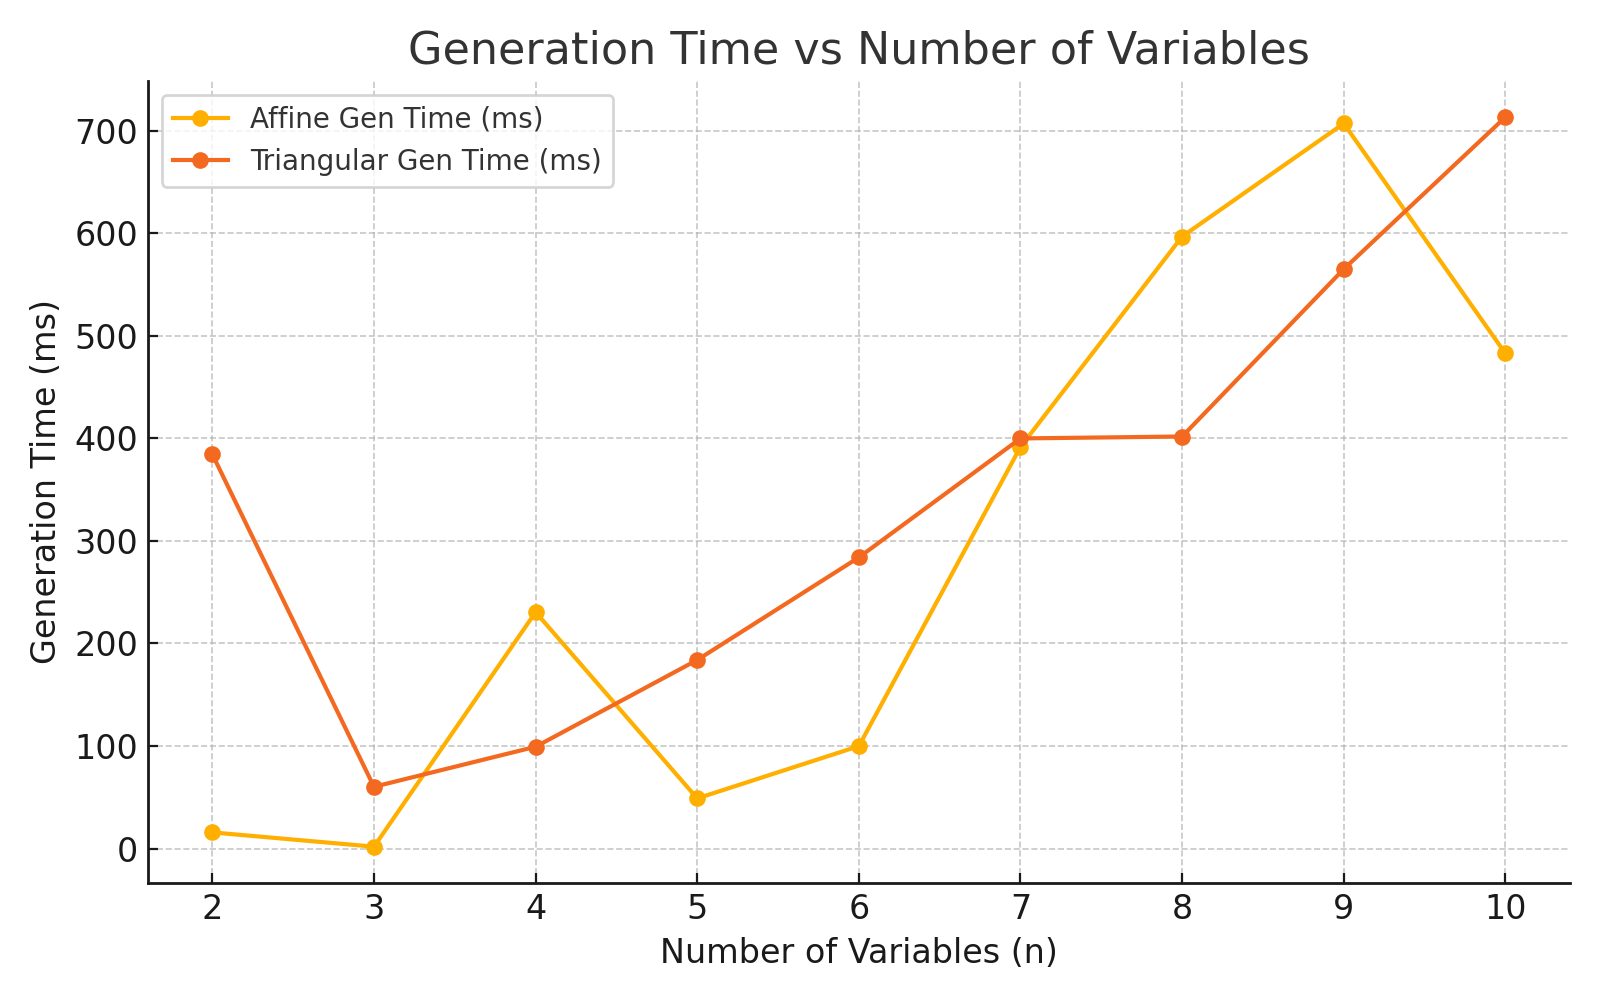
\includegraphics[width=\textwidth]{benchmark_plot.png}
        \caption{Runtime plot of map generation}
    \end{subfigure}

    \vspace{1em}

    \begin{subfigure}{0.85\textwidth}
        \centering
        \renewcommand{\arraystretch}{1.3}
        \begin{tabularx}{\textwidth}{|X|X|X|}
            \hline
            \textbf{Number of variables, $n$} & \textbf{Triangular (ms)} & \textbf{Affine (ms)} \\
            \hline
            3 & 0.3 & 0.1 \\
            5 & 1.2 & 0.3 \\
            7 & 3.8 & 1.0 \\
            \hline
        \end{tabularx}
        \caption{Average generation time for affine and triangular maps as a function of \( n \).}
    \end{subfigure}

    \caption{Benchmark results showing runtime and average generation time for affine and triangular maps over \( \mathbb{Z}_p \).}
    \label{fig:benchmark-plot}
\end{figure}
\footnotemark
\footnotetext{Benchmarks were run using Python 3.10 on an Intel(R) Core(TM) i7 CPU with 16 GB RAM under Ubuntu 22.04, single thread. Results averaged over 5 runs.}

\section*{Supplementary Materials}

The full source code for our cryptosystem is available at:

\begin{quote}
\url{https://github.com/SAIMON-AHMED/jacobian-crypto-composition}

\end{quote}

This repository includes:
\begin{itemize}
    \item Polynomial map generators (affine and triangular),
    \item Streamlit-based graphical interface (`app/`),
    \item Benchmarking and performance scripts (`benchmark/`),
    \item Worked examples, tests, and invertibility checks (`tests/`),
    \item MIT License for open-source usage,
    \item All dependencies specified in \texttt{requirements.txt}.
\end{itemize}




\section{Future Work and Generalizations}

\begin{itemize}
    \item \textbf{Generalizing to Wild Automorphisms:}  
    Our construction is currently limited to tame automorphisms — compositions of triangular and affine polynomial maps. However, the Jacobian condition \( \det J = 1 \) is also satisfied by certain wild automorphisms. Future work may explore the cryptographic suitability of wild maps, such as the famous Nagata automorphism in dimension 3, and test their obfuscation properties under composition.

    \item \textbf{Higher-Order Composition Patterns:}  
    We plan to study more complex composition hierarchies (e.g., alternating affine/triangular stacks) and analyze how they affect invertibility, key size, and obfuscation quality.

    \item \textbf{Integration with Key Encapsulation Mechanisms (KEMs):}  
    Our system could be adapted for hybrid encryption by embedding it into a KEM structure. This would make the scheme more compatible with modern public-key encryption frameworks.
\end{itemize}


\section{Conclusion}

We have introduced a novel public-key cryptosystem based on the Jacobian conjecture and the composition of invertible polynomial maps over finite fields. By constructing the public key as a composition \( H = f_1 \circ f_2 \circ \dots \circ f_k \) of triangular and affine polynomial maps with Jacobian determinant equal to 1, we ensure guaranteed invertibility while simultaneously introducing algebraic complexity. Our system is designed to resist both classical and quantum attacks by leveraging the computational hardness of symbolic inversion and polynomial decomposition. Through formal correctness proofs, worked examples, and a Python-based implementation, we provide a practical and theoretically grounded framework for post-quantum cryptography. Future work includes generalizing to more exotic map classes and performing formal cryptanalysis under advanced algebraic models.

\section*{Acknowledgments}
The author would like to thank Professor Lavinia Ciungu (Department of Mathematics, St. Francis College) for valuable guidance, support, and feedback during the development of this work.


\section*{References}
\begin{thebibliography}{99}


\bibitem{Bass1982}
Hyman Bass, Edwin H. Connell, and David Wright, 
\textit{The Jacobian Conjecture: Reduction of Degree and Formal Expansion of the Inverse}, 
Bulletin of the American Mathematical Society, vol. 7, no. 2, 1982, pp. 287–330.

\bibitem{Essen2000}
Arno van den Essen, 
\textit{Polynomial Automorphisms and the Jacobian Conjecture}, 
Progress in Mathematics, vol. 190, Birkhäuser, 2000.

\bibitem{Dubrovin2018}
Boris A. Dubrovin, 
\textit{Modern Geometry — Methods and Applications Part III: Introduction to Homology Theory}, 
Springer, 2018.

\bibitem{Ding2004}
Jintai Ding et al.,
\textit{Multivariate Public Key Cryptosystems}, 
in Post-Quantum Cryptography, Springer, 2004.

\bibitem{Koblitz1994}
Neal Koblitz, 
\textit{A Course in Number Theory and Cryptography}, 
2nd ed., Springer-Verlag, 1994.

\bibitem{Cox2007}
David Cox, John Little, Donal O'Shea,
\textit{Ideals, Varieties, and Algorithms: An Introduction to Computational Algebraic Geometry and Commutative Algebra}, 
Springer, 2007.

\bibitem{Patarin1996}
Jacques Patarin, 
\textit{Hidden Field Equations (HFE) and Isomorphisms of Polynomials (IP): Two new families of asymmetric algorithms}, 
EUROCRYPT 1996, Springer, pp. 33–48.

\bibitem{Rainbow}
Jintai Ding and Dieter Schmidt, 
\textit{Rainbow, a new multivariable polynomial signature scheme}, 
ACNS 2005, Springer, pp. 164–175.

\bibitem{FaugereF5}
Jean-Charles Faugère, 
\textit{A new efficient algorithm for computing Gröbner bases without reduction to zero (F5)}, 
Proceedings of the 2002 international symposium on Symbolic and algebraic computation (ISSAC), ACM, 2002.

\bibitem{Beullens2022}
Ward Beullens,
\textit{Breaking Rainbow Takes a Weekend on a Laptop}, 
In Advances in Cryptology – EUROCRYPT 2022, pp. 507–536.


\end{thebibliography}


\end{document}
